%!TEX program = xelatex
\documentclass{beamer}

\usepackage{booktabs}
\usepackage{pifont}
\usepackage{rotating}
\usepackage{appendixnumberbeamer}
\usepackage[caption=false]{subfig}

\usetheme{Execushares}

\title{Numerical Characterization of Ultrasound Elastography for the Early Detection of Deep Tissue Injuries}
\subtitle{A thesis submitted in partial fulfilment of the requirements for the degree of Master of Science}
\author{Kenton David Hamaluik}
\institute{University of Alberta}
\date{June 23, 2014}

\newcommand{\rotHead}[1]{\begin{rotate}{60}#1\end{rotate}}
\newcommand{\cmark}{\color{ExecusharesBlue}\ding{51}}
\newcommand{\xmark}{\color{ExecusharesRed}\ding{55}}

\setcounter{showSlideNumbers}{1}

\begin{document}

	\frame{\titlepage}

	\begin{frame}
		\frametitle{Contents}
		\begin{enumerate}
			\item Introduction \\ \textcolor{ExecusharesGrey}{\footnotesize\hspace{1em} The reasons for and goals of this research}
			\item Quasi-Static Ultrasound Elastography (\alert{QS USE}) \\ \textcolor{ExecusharesGrey}{\footnotesize\hspace{1em} Estimating stiffness using manual palpation}
			\item Acoustic Radiation Force Impulse (\alert{ARFI}) Imaging \\ \textcolor{ExecusharesGrey}{\footnotesize\hspace{1em} Using transducer-generated forces instead of manual palpation}
			\item Shear Wave Speed Quantification \\ \textcolor{ExecusharesGrey}{\footnotesize\hspace{1em} Quantifying tissue stiffness using shear wave speeds}
			\item Conclusions \\ \textcolor{ExecusharesGrey}{\footnotesize\hspace{1em} Recommendations and final thoughts}
		\end{enumerate}
	\end{frame}

	\setcounter{framenumber}{0}
	\section{Introduction}
		\begin{frame}
			\frametitle{Pressure Ulcers}
			\begin{columns}[c]
				\column{0.45\textwidth}
				\begin{itemize}
					\item Pressure ulcers are secondary injuries
					\begin{itemize}
						\item People with reduced mobility
					\end{itemize}

					\item Skin breakdown due to moisture, shear / friction

					\item Categorized by NPUAP in stages
					\begin{itemize}
						\item From shallow to deep
					\end{itemize}
				\end{itemize}

				\column{0.55\textwidth}
					\begin{figure}
						\centering
						\subfloat{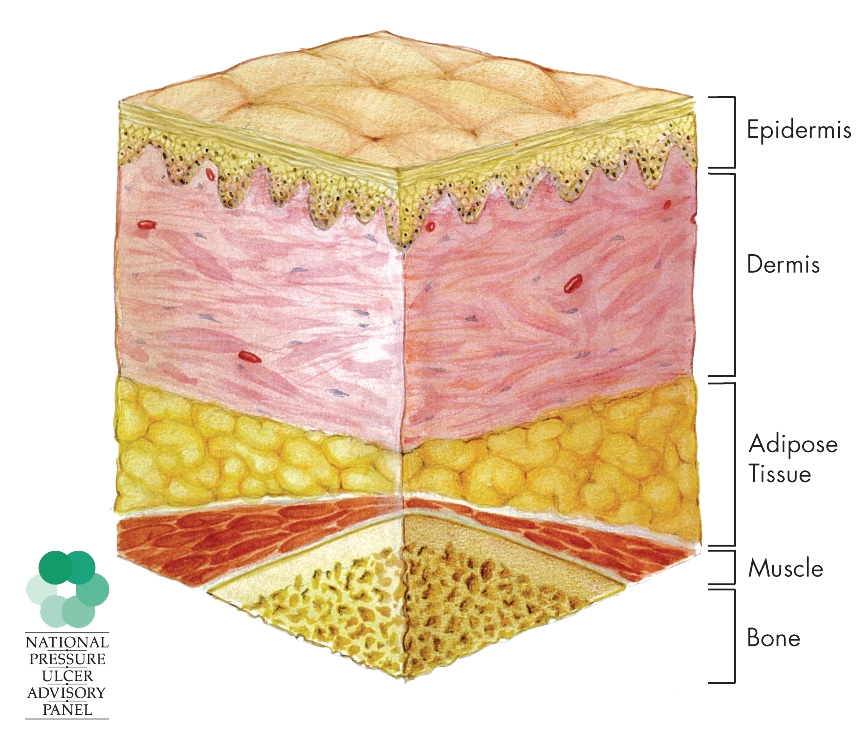
\includegraphics[width=0.33\textwidth]{assets/npuap/normal.png}}

						\subfloat{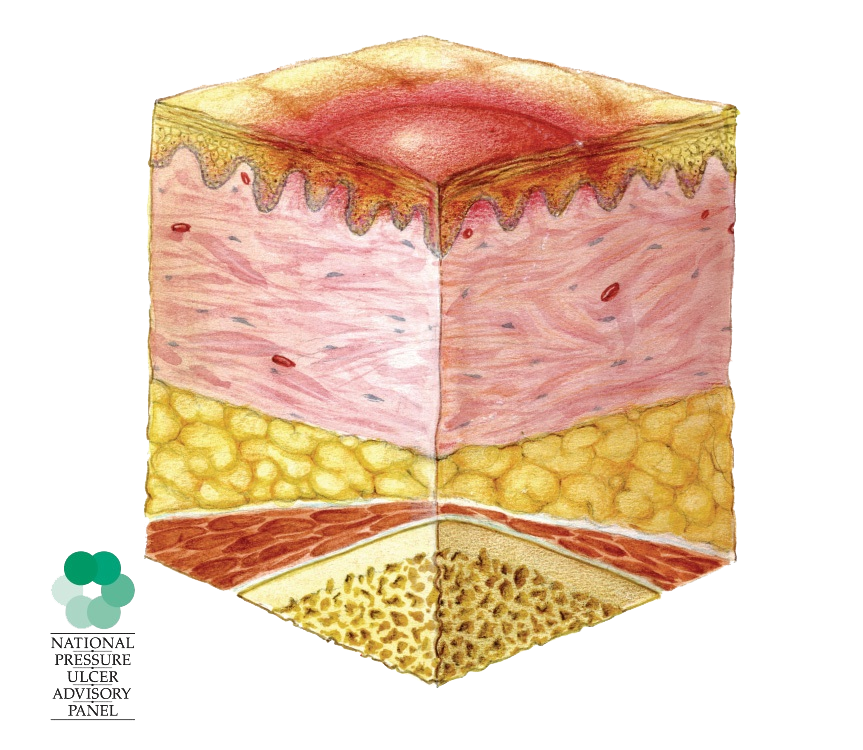
\includegraphics[width=0.33\textwidth]{assets/npuap/stage1.png}}
						\subfloat{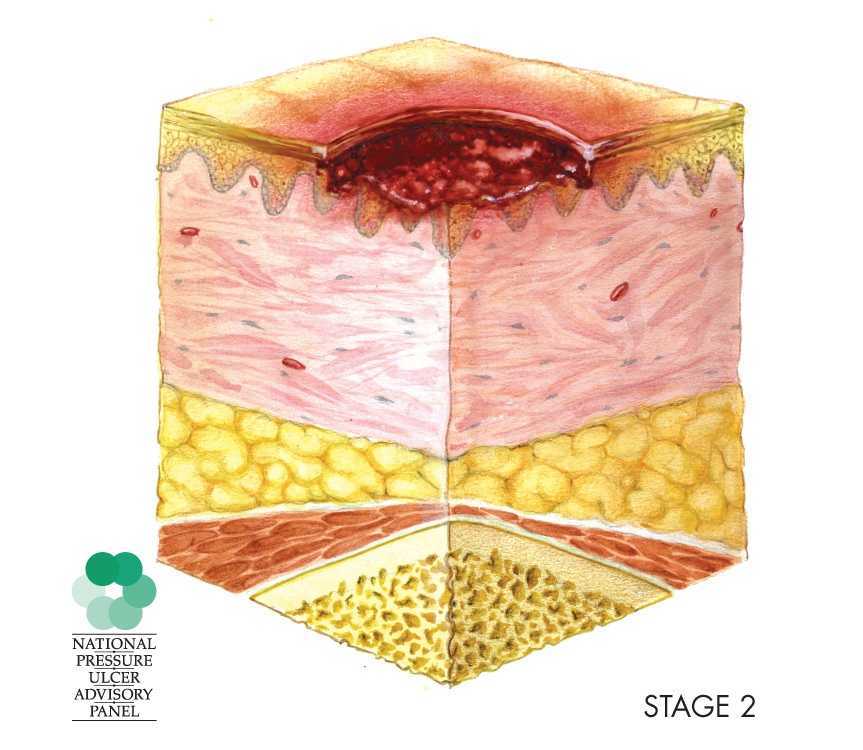
\includegraphics[width=0.33\textwidth]{../latex/assets/npuap/stage2.png}}
						\subfloat{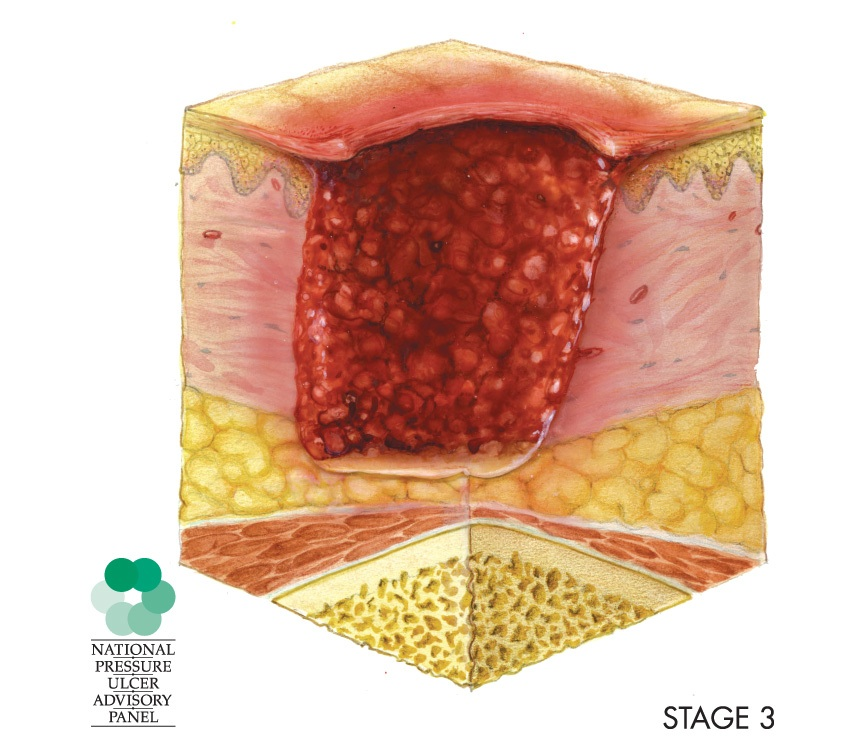
\includegraphics[width=0.33\textwidth]{../latex/assets/npuap/stage3.png}}

						\subfloat{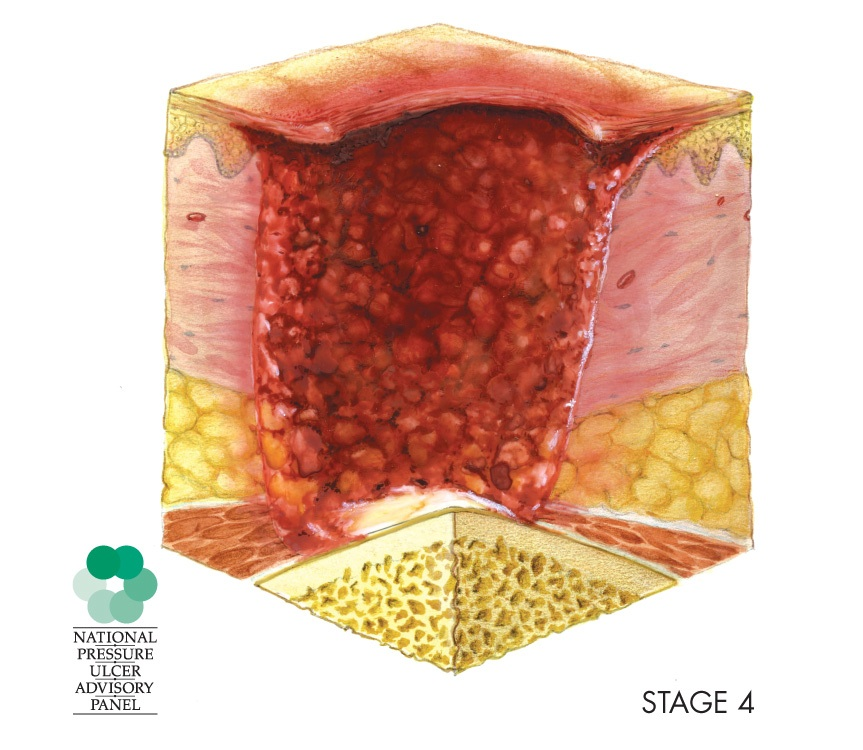
\includegraphics[width=0.33\textwidth]{../latex/assets/npuap/stage4.png}}
						\subfloat{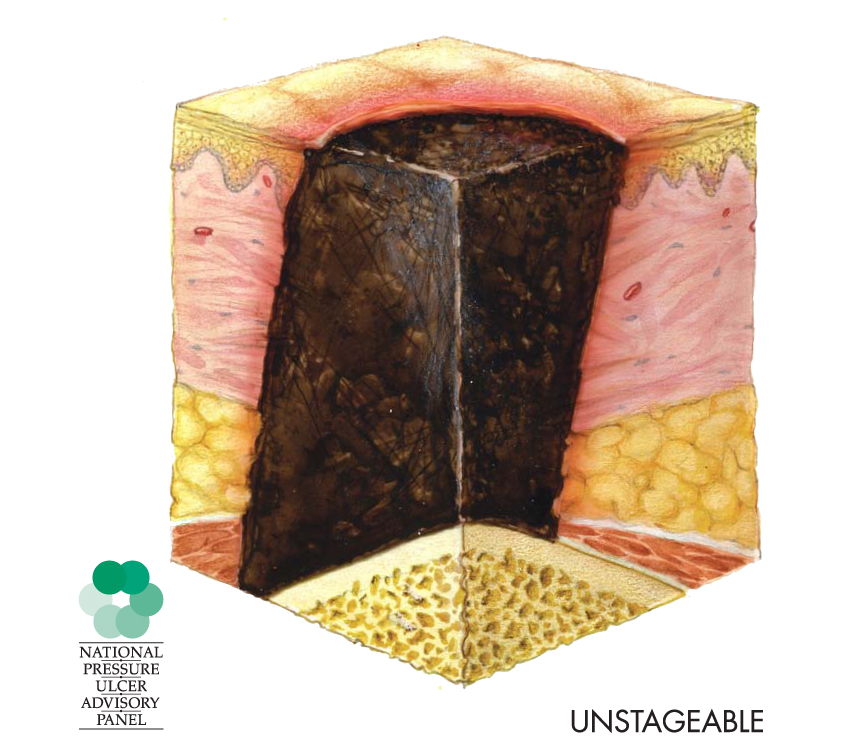
\includegraphics[width=0.33\textwidth]{../latex/assets/npuap/unstageable.png}}
						\subfloat{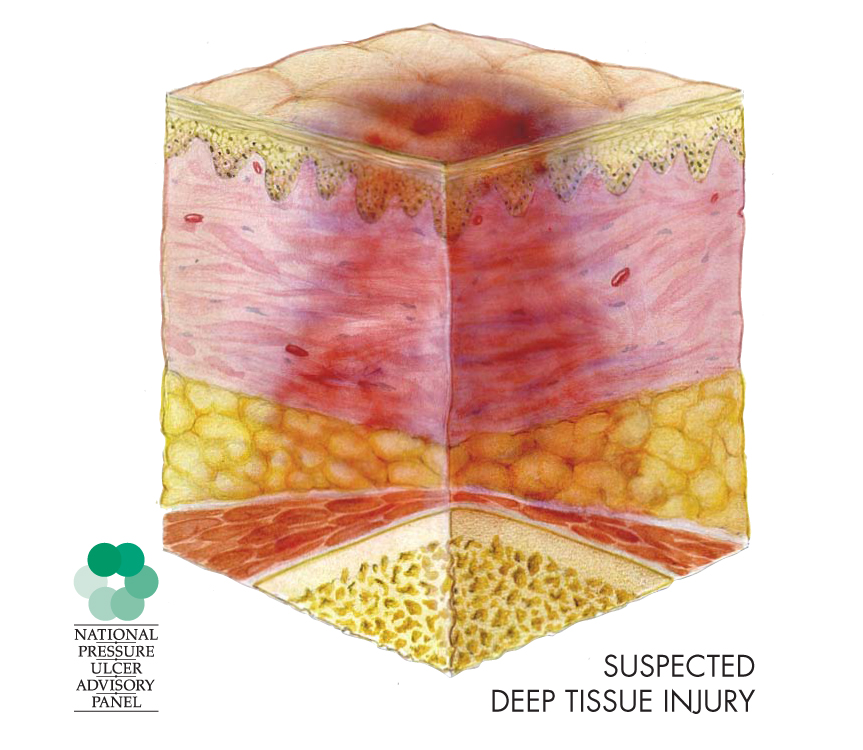
\includegraphics[width=0.33\textwidth]{../latex/assets/npuap/suspectedDTI.png}}

						\caption{\copyright\ National Pressure Ulcer Advisory Panel, used with permission.}
					\end{figure}
			\end{columns}
		\end{frame}

		\begin{frame}
			\frametitle{Deep Tissue Injuries}
			\begin{columns}[c]
				\column{0.65\textwidth}
				\begin{itemize}
					\item Not all PU form ``top-to-bottom''
					\begin{itemize}
						\item Deep tissue injuries (\alert{DTI}) form ``bottom-to-top''
						\item Eventually break out into stage III -- IV pressure ulcers
					\end{itemize}

					\item Tissue damage due to pressure and deformation

					\item Almost impossible to detect clinically
				\end{itemize}

				\column{0.35\textwidth}
					\begin{figure}
						\centering
						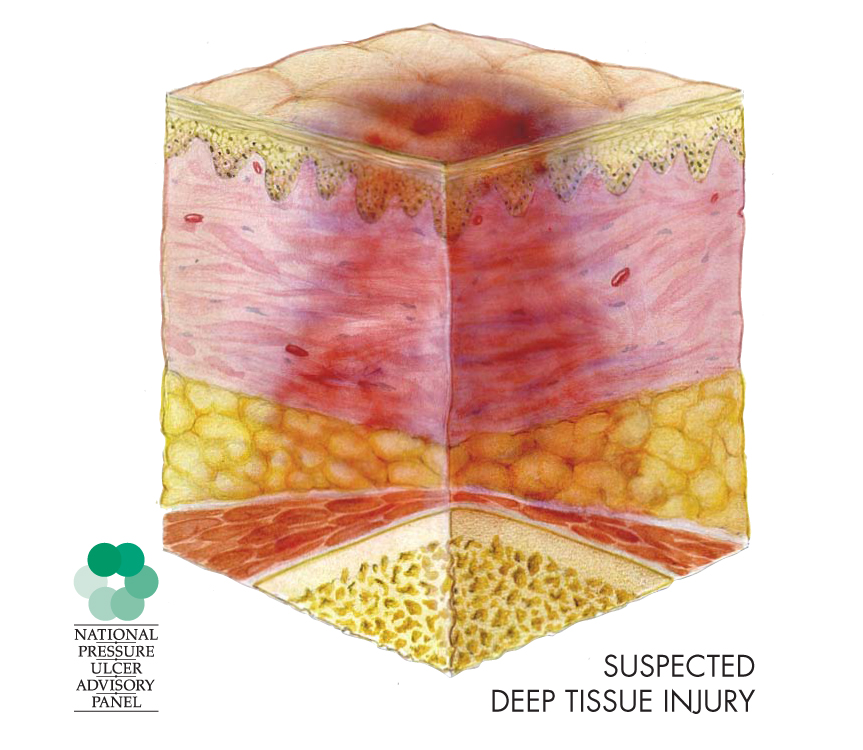
\includegraphics[width=\textwidth]{../latex/assets/npuap/suspectedDTI.png}

						\caption{\copyright\ National Pressure Ulcer Advisory Panel, used with permission.}
					\end{figure}
			\end{columns}
		\end{frame}

		\begin{frame}
			\frametitle{Deep Tissue Injury Detection}
			\begin{itemize}
				\item T$_2^*$-weighted MRI in research settings
				\item Risk assessment scales in clinical settings
				\begin{itemize}
					\item Norton, Braden, and Risk Assessment Pressure Sore scales
				\end{itemize}
			\end{itemize}
		\end{frame}

		\begin{frame}
			\frametitle{Filling the Gaps}
			\begin{center}
				\vspace{1cm}
				\begin{tabular}{r|ccccccccccc}
					& \rotHead{DTI} & \rotHead{B-Mode} & \rotHead{QS USE} & \rotHead{ARFI} & \rotHead{Shear} & \rotHead{FEM} & \rotHead{Phantom} & \rotHead{Animals} & \rotHead{Humans} & \rotHead{Characterization} & \rotHead{Clinical} \\
					\hline
					PU Risk scales & \xmark & \xmark & \xmark & \xmark & \xmark & \xmark & \xmark & \xmark & \cmark & \xmark & \cmark \\
					T$_2^*$ MRI & \cmark & --- & --- & --- & --- & \cmark & \cmark & \cmark& \cmark & \xmark & \xmark \\
					Aoi et al. & \cmark & \cmark & \xmark & \xmark & \xmark & \xmark & \xmark & \xmark & \cmark & \xmark & \cmark\emph{\textbf{*}} \\
					Deprez et al. & \cmark & \xmark & \cmark & \xmark & \xmark & \cmark & \cmark & \cmark & \xmark & \xmark & \cmark \\
					This work & \cmark & \xmark & \cmark & \cmark & \cmark & \cmark & \cmark & \xmark & \xmark & \cmark & \cmark \\
				\end{tabular}
			\end{center}
		\end{frame}

		\begin{frame}
			\frametitle{What?}
		\end{frame}

	\section[QS USE]{Quasi-Static Ultrasound Elastography}
		\begin{frame}
			\frametitle{Introduction}
		\end{frame}

	\section[ARFI]{Acoustic Radiation Force Impulse Imaging}
		\begin{frame}
			\frametitle{Introduction}
		\end{frame}

	\section[Shear]{Shear Wave Speed Quantification}
		\begin{frame}
			\frametitle{Introduction}
		\end{frame}

	\section{Conclusions}
		\begin{frame}
			\frametitle{Comparing Methods}
		\end{frame}
		\begin{frame}
			\frametitle{Recommendations}
		\end{frame}

	\appendix
	\section{Additional Slides}
	\setcounter{showProgressBar}{0}
	\setcounter{showSlideNumbers}{0}

		\begin{frame}
			\frametitle{Additional Slides}
			\begin{itemize}
				\item \hyperlink{backup1}{backup 1}
			\end{itemize}
		\end{frame}

		\begin{frame}[label=backup1]
			\frametitle{backup1}
			\begin{itemize}
				\item herp
			\end{itemize}
		\end{frame}

\end{document}